% cpu/cpu.tex
% mainfile: ../perfbook.tex
% SPDX-License-Identifier: CC-BY-SA-3.0

\QuickQuizChapter{chp:Hardware and its Habits}{硬件及其特性}{qqzcpu}
%
\Epigraph{过早抽象是万恶之源。}
	 {众人之见}

大多数人凭直觉就能理解，在系统之间传递消息比在单个系统内部执行简单计算要昂贵得多。
但同样需要认识到的是，在单个共享内存系统内部的线程（thread）之间进行通信也可能相当昂贵。
因此，本章将探讨共享内存系统内部同步和通信的开销。
这寥寥数页只能触及共享内存并行硬件设计的皮毛；希望深入了解的读者不妨从
\pplsur{John L.}{Hennessy}和\pplsur{David A.}{Patterson}的经典教材的
最新版本~\cite{Hennessy2017}开始阅读。

\QuickQuiz{
	为什么并行程序员要费心学习硬件的底层特性？
	保持在更高的抽象层次上难道不是更容易、更好、更优雅、更高效吗？
}\QuickQuizAnswer{
	忽略硬件的具体特性通常确实更容易，更高层次的抽象也确实能大大提高生产力。
	但对于我们这些从事底层并发软件的人来说，忽视这些特性是相当愚蠢的。

	毕竟，如果你承认并行的唯一目的是提升性能，
	并且进一步承认性能取决于硬件的具体特性，
	那么合乎逻辑的结论就是：并行程序员至少需要了解一些硬件特性。

	在大多数工程学科中也是如此。
	\emph{你}愿意使用一位不了解构成桥梁的混凝土和钢材特性的
	工程师所设计的桥梁吗？
	如果不愿意，那你为什么期望一个并行程序员在对底层硬件
	\emph{毫无}了解的情况下，能够开发出合格的并行软件呢？

	简而言之，你可以不关心物理定律，但物理定律非常关心你的代码！
}\QuickQuizEnd

% cpu/overview.tex
% mainfile: ../perfbook.tex
% SPDX-License-Identifier: CC-BY-SA-3.0

\section{概述}
\label{sec:cpu:Overview}
%
\epigraph{机械同理心：硬件与软件和谐协作。}
	 {Martin Thompson}

如果只是粗略地扫一眼计算机系统的规格表，人们很容易觉得CPU的性能就像在一条平坦赛道上赛跑，
如\cref{fig:cpu:CPU Performance at its Best}所示，
总是跑得最快的选手赢得比赛。

\begin{figure}
\centering
\resizebox{3in}{!}{\includegraphics{cartoons/r-2014-CPU-track-meet}}
\caption{CPU最佳性能表现}
\ContributedBy{fig:cpu:CPU Performance at its Best}{Melissa Broussard}
\end{figure}

虽然确实存在少数针对CPU的benchmark能够接近
\cref{fig:cpu:CPU Performance at its Best}中所示的理想情况，
但典型的程序与其说是赛跑，更不如说是障碍赛。
托\IXr{Moore's Law}的福，过去几十年间CPU的内部架构发生了急剧变化。
以下各节将介绍其中一些架构变化。

\subsection{流水线CPU}
\label{sec:cpu:Pipelined CPUs}

\begin{figure}
\centering
\resizebox{3in}{!}{\includegraphics{cartoons/r-2014-Old-man-and-Brat}}
\caption{新旧CPU}
\ContributedBy{fig:cpu:CPUs Old and New}{Melissa Broussard}
\end{figure}

在1980年代，典型的微处理器在处理下一条指令之前，至少需要取指、解码和执行
三个时钟周期来完成当前指令。
相比之下，1990年代末和2000年代的CPU可以同时处理许多条指令，
使用\emph{流水线}、\emph{超标量}技术、\emph{乱序}指令和数据处理、
\emph{推测执行}等更多技术~\cite{Hennessy2017}来优化指令和数据
在CPU中的流动。
一些核心拥有多个硬件线程，这被称为
\emph{同步多线程}（SMT）或\emph{超线程}
（HT）~\cite{JFennel1973SMT}，
每个硬件线程在软件看来都是一个独立的CPU，至少从功能角度来看是这样。
这些现代硬件特性可以极大地提升性能，
如\cref{fig:cpu:CPUs Old and New}所示。

带有长流水线的CPU要达到最佳性能，需要程序具有高度可预测的控制流。
如果程序的主要代码是在执行紧凑循环，那么就能提供这样的控制流，
例如对大型矩阵或向量进行算术运算的程序。
此时CPU可以正确预测出在大多数情况下循环末尾的分支走向，
从而保持流水线满载，让CPU全速运行。

\begin{figure}
\centering
\resizebox{3in}{!}{\includegraphics{cartoons/r-2014-branch-error}}
\caption{CPU遭遇流水线冲刷}
\ContributedBy{fig:cpu:CPU Meets a Pipeline Flush}{Melissa Broussard}
\end{figure}

然而，分支预测并不总是那么容易。
例如，如果程序中带有许多循环，且每个循环的迭代计数都比较小，
或者面向对象的程序中带有许多虚方法，每个虚方法都可以引用不同的对象实例，
而这些对象实例都实现了一些频繁被调用的成员函数，
此时CPU很难甚至完全不可能预测某个分支的走向。
这样CPU要么等待控制流进行到足以知道分支走向的地步，
要么干脆猜测并使用推测执行继续前进。
虽然猜测对于控制流可预测的程序效果极好，
但对于不可预测的分支（如二分搜索中的分支），
CPU常常猜错。
一次错误的猜测代价很高，因为CPU必须丢弃错误分支之后所有
推测执行的指令，导致流水线冲刷。
如果流水线冲刷发生得过于频繁，就会大幅降低整体性能，
如\cref{fig:cpu:CPU Meets a Pipeline Flush}中所夸张描绘的那样。

\begin{figure}
\centering
\resizebox{3in}{!}{\includegraphics{cpu/microarch}}
\caption{现代微架构概略图}
\label{fig:cpu:Rough View of Modern Micro-Architecture}
\end{figure}

对于超线程（或SMT，如果你更喜欢这个叫法的话）来说情况更糟，
特别是在具有推测执行功能的流水线超标量乱序CPU上。
在这种日益常见的情况下，共享一个核心的所有硬件线程也共享该核心的资源，
包括寄存器、cache、执行单元等等。
指令通常被解码为微操作，共享执行单元和数百个硬件寄存器的使用通常
由一个微操作调度器来协调。
这样一个双线程核心的概略图如
\cref{fig:cpu:Rough View of Modern Micro-Architecture}所示，
更精确（因而也更复杂）的图可以在教科书和学术论文中找到。\footnote{
	这是一个2010年代末的Intel核心的示例：
	\url{https://en.wikichip.org/wiki/intel/microarchitectures/skylake_(server)}。}
因此，一个硬件线程的执行可能而且经常会受到共享同一核心的
其他硬件线程的行为的干扰。

即使只有一个硬件线程处于活动状态（例如，在只有一个线程的
传统CPU设计中），反直觉的结果也相当常见。
执行单元往往具有重叠的功能，因此CPU对执行单元的选择
可能会导致流水线停顿，因为后续指令会争用该执行单元。
理论上这种争用是可以避免的，但实际上CPU必须非常快速地做出选择，
且无法预知未来。
特别值得注意的是，向一个紧密循环中添加一条指令，
有时反而会使执行\emph{加速}。

不幸的是，流水线冲刷和共享资源争用并不是现代CPU在其
障碍赛道上面临的唯一风险。
下一节将介绍内存引用的相关风险。

\subsection{内存引用}
\label{sec:cpu:Memory References}

在1980年代，微处理器从内存读取一个值的时间通常比执行一条指令还短。
而在较近的时期，同样是读取内存里一个值的时间，微处理器可以执行数百甚至数千条指令。
这种差距主要源于\IXr{Moore's Law}使得CPU性能的增长速度大大超过
内存\IX{latency}的降低速度，也有部分来源于内存容量的增长速度。
例如，1970年代的典型小型计算机通常只有4\,KB
（是的，是千字节，不是兆字节，更别提吉字节或太字节了）的主存，
且访问只需一个CPU周期。\footnote{
	公平地说，这些单周期中的每一个周期都不少于1.6\emph{微秒}。}
如今的CPU设计师仍然可以设计出单周期访问的4\,KB内存，
即使在具有多GHz时钟频率的系统上也是如此。
事实上他们确实经常设计这样的内存，只不过现在称之为
``零级cache''，容量也大大超过4\,KB。

\begin{figure}
\centering
\resizebox{3in}{!}{\includegraphics{cartoons/r-2014-memory-reference}}
\caption{CPU遭遇内存引用}
\ContributedBy{fig:cpu:CPU Meets a Memory Reference}{Melissa Broussard}
\end{figure}

虽然现代微处理器上的大容量cache极大地减少了内存访问延迟，
但只有高度可预测的数据访问模式才能让cache发挥最大效用。
不幸的是，像遍历链表这样的常见操作具有极其不可预测的内存访问模式——
毕竟，如果这些模式是可预测的，我们也就不会被指针所困扰了，对吧？
因此，如\cref{fig:cpu:CPU Meets a Memory Reference}所示，
内存引用往往对CPU性能造成严重影响。

到目前为止，我们只考虑了给定CPU在执行单线程代码时可能遇到的障碍。
多线程给CPU带来了额外的障碍，如以下各节所述。

\subsection{原子操作}
\label{sec:cpu:Atomic Operations}

还有一种障碍是\IX{atomic}操作。
原子操作（atomic operation）的概念在某种意义上与CPU流水线一次执行多条指令的
运作方式相冲突。
拜硬件设计者的精密设计所赐，现代CPU使用了许多极其巧妙的技巧使这些操作
\emph{看起来}是原子的，尽管它们实际上是逐步执行的。
一个常见的技巧是：标出所有包含原子操作所需数据的cache line，
确保CPU在执行原子操作时这些cache line都归该CPU所有，
并且只有在这些cache line仍归该CPU所有时才推进原子操作的执行。
这样一来，因为所有数据都只属于该CPU，即使CPU的流水线可以同时执行多条指令，
其他CPU也无法干扰此CPU的原子操作执行。
不用多说，这种技巧要求流水线必须能被延迟甚至冲刷，
才能执行让原子操作正确完成的一系列准备操作。

\begin{figure}
\centering
\resizebox{3in}{!}{\includegraphics{cartoons/r-2014-Atomic-reference}}
\caption{CPU遭遇原子操作}
\ContributedBy{fig:cpu:CPU Meets an Atomic Operation}{Melissa Broussard}
\end{figure}

非原子操作则与之相反，CPU可以从cache line中按照数据到达的顺序加载值，
并将结果放入store buffer中，无需等待cache line的所有权切换。
虽然有一些硬件优化有时可以隐藏cache延迟，
但原子操作对性能的影响往往如
\cref{fig:cpu:CPU Meets an Atomic Operation}所描绘的那样。

不幸的是，原子操作通常只适用于单个数据元素。
由于许多并行算法要求在多个数据元素的更新之间维持排序约束，
大多数CPU提供了memory barrier。
这些memory barrier也是性能消耗的障碍，如下一节所述。

\QuickQuiz{
	什么类型的机器能够对多个数据元素执行原子操作？
}\QuickQuizAnswer{
	一个答案是，通常可以将多个数据元素打包到一个机器字中，
	然后对其进行原子操作。

	一个更时髦的答案是支持事务内存（transactional memory）的
	机器~\cite{DBLomet1977SIGSOFT,Knight:1986:AMF:319838.319854,Herlihy93a}。
	到2014年初，几个主流系统提供了有限的硬件事务内存实现，
	其优缺点在\cref{sec:future:Hardware Transactional Memory}中有更详细的介绍。
	关于软件事务内存的适用性，业界也尚未定论~\cite{McKenney2007PLOSTM,DonaldEPorter2007TRANSACT,
	ChistopherJRossbach2007a,CalinCascaval2008tmtoy,
	AleksandarDragovejic2011STMnotToy,AlexanderMatveev2012PessimisticTM}，
	相关内容在\cref{sec:future:Transactional Memory}中有所介绍。
}\QuickQuizEnd

\subsection{内存屏障（memory barrier）}
\label{sec:cpu:Memory Barriers}

\IXpl{Memory barrier}将在
\cref{chp:Advanced Synchronization: Memory Ordering}和
\cref{chp:app:whymb:Why Memory Barriers?}中更详细地讨论\@。
在此期间，考虑以下简单的基于lock的\IX{critical
section}：

\begin{VerbatimN}[samepage=true]
spin_lock(&mylock);
a = a + 1;
spin_unlock(&mylock);
\end{VerbatimN}

\begin{figure}
\centering
\resizebox{3in}{!}{\includegraphics{cartoons/r-2023-Memory-barrier}}
\caption{CPU遭遇Memory Barrier}
\ContributedBy{fig:cpu:CPU Meets a Memory Barrier}{Melissa Broussard}
\end{figure}

如果CPU没有按照上述语句的顺序执行，
变量``a''就会在没有``mylock''保护的情况下被递增，
这肯定和我们获取锁的目的不一致。
为了防止这种有害的乱序执行，锁操作原语中必须包含显式或隐式的memory barrier。
由于memory barrier的作用就是阻止CPU（更不用说编译器）
为了提高性能而进行的乱序执行，
所以memory barrier几乎总是会降低性能，
如\cref{fig:cpu:CPU Meets a Memory Barrier}所描绘的那样。

与原子操作一样，CPU设计师一直在努力降低\IXh{memory-barrier}{overhead}，
并已取得了实质性进展。

\subsection{功能单元的不足}
\label{sec:cpu:Functional Unit Failings}

现代超标量CPU拥有众多用途和能力各异的功能单元。
每个CPU可能有多个用于整数和布尔运算的算术逻辑单元（ALU）、
几个向量单元、几个浮点单元（FPU），以及至少各一个的分支单元、
加载单元和存储单元。
不同的CPU当然会有不同的功能单元组合。
然而，不仅不同的应用程序需要不同的功能单元组合，
给定的应用程序在不同的执行阶段也可能需要不同的组合。

\begin{figure}
\centering
\resizebox{2.5in}{!}{\includegraphics{cartoons/CPU-track-meet-functional-units}}
\caption{CPU功能单元不匹配}
\ContributedBy{fig:cpu:CPU Functional-Unit Mismatch}{Melissa Broussard, remixed}
\end{figure}

这意味着，认为某个CPU拥有完美的功能单元组合并没有太大意义。
有时候CPU反而必须``单脚跳着走''，只使用其令人印象深刻的功能单元
阵列中的极少数几个，
如\cref{fig:cpu:CPU Functional-Unit Mismatch}中输掉比赛的
那个不幸的CPU所夸张描绘的那样。

\QuickQuiz{
	但这与在多核CPU上扩展工作负载有什么关系？
}\QuickQuizAnswer{
	在很多情况下，关系相当大！
	例如，在具有超线程核心的系统上，共享一个核心的硬件线程也共享
	其功能单元，这可能导致另一种形式的争用，从而限制可扩展性。
	再举一个例子，拥有令人印象深刻的功能单元阵列的全部意义在于
	支持指令级并行，即CPU内部的并发性和可扩展性。
}\QuickQuizEnd

不幸的是，即使一个工作负载能完美高效地使用给定CPU的每一个功能单元，
它仍然可能失败，例如下一节所描述的情况。

\subsection{热节流}
\label{sec:cpu:Thermal Throttling}

一种越来越常见的令人沮丧的经历是：精心微优化一段关键代码路径，
大幅减少了该代码路径消耗的时钟周期数，
却发现该代码消耗的挂钟时间实际上\emph{增加}了。

\begin{figure}
\centering
\resizebox{3in}{!}{\includegraphics{cartoons/r-2022-Thermal-throttling}}
\caption{CPU遭遇热节流}
\ContributedBy{fig:cpu:Encounters Thermal Throttling}{Melissa Broussard, remixed}
\end{figure}

欢迎来到现代\IX{thermal throttling}的世界。

如果你通过更高效地利用CPU的功能单元来减少时钟周期数，
你就会增加该CPU消耗的功率。
这反过来会增加该CPU散发的热量。
如果这些热量超出了散热系统的能力，系统就会对该CPU进行热节流，
例如降低其时钟频率，
如\cref{fig:cpu:Encounters Thermal Throttling}中的雪企鹅
所夸张描绘的那样。

如果性能至关重要，正确的修复方法是改善散热，
这种方法受到硬核玩家、超频爱好者
（其中一些人善于利用液氮）以及性能优先的系统供应商
（其中有一家使用每CPU一个铝制散热器，每个重达一磅，即0.454公斤）的青睐。
但如果你无法修改计算机的散热系统，
例如因为你是从云服务提供商租用的，
那么你就需要采取其他优化方法。
例如，你可能需要应用算法优化而非以硬件为中心的微优化。
或者，你可以将代码并行化，将工作（因而也是热量）分散到多个CPU核心上。

有些人建议根据各种CPU核心时钟频率来归一化给定测试的结果，
这可能有所帮助。
然而，cache miss和内存访问的延迟并不依赖于CPU核心时钟频率。
此外，如果被测代码涉及多个CPU之间的紧密交互，
那么在一个CPU上运行的代码的性能将取决于其他CPU的核心时钟频率。

最后，如果目标是获得可重复的benchmark测量结果，
一种方法是将传统的cache预热扩展为包括热预热，
所需的预热时间取决于被测系统的大小，因而也取决于其热惯性。

另一种可重复benchmark的方法适用于基于事件的应用程序，
这些程序以短暂但间隔很大的突发形式运行对延迟敏感的执行。
在这种情况下，前述方法的热预热间隔应替换为冷却间隔，
在此期间系统保持空闲。

即使经过了仔细的热预热或冷却，结果仍可能随环境温度的变化而变化，
而环境温度可能强烈依赖于一天中的时段，
更不用说世界某些地区的季节了。

\QuickQuiz{
	在热预热或冷却时间较长且工作负载固定的情况下，
	为什么环境温度会有影响？
}\QuickQuizAnswer{
	是的，以固定CPU核心时钟频率运行的固定工作负载
	确实可能产生恒定的热流，
	尽管在创建CPU热模型时面临许多挑战。
	然而，环境温度越低，热量从CPU流向周围环境的速度就越快。
	这反过来，加上恒定的热流，意味着较低的环境温度将导致较低的CPU温度，
	从而减少热节流。
	因此，给定的benchmark在夜间或冬季可能会产生更高的性能，
	也就是环境温度趋于较低的时候。
}\QuickQuizEnd

\subsection{缓存未命中（cache miss）}
\label{sec:cpu:Cache Misses}

对多线程程序来说，还有一个额外的障碍影响CPU性能——``cache miss''。
正如前文提到的，现代CPU使用大容量cache来降低由于较高的内存访问延迟带来的性能损失。
但是，对于在多个CPU间频繁共享的变量，cache事实上起到了反效果。
因为当某个CPU想去修改该变量时，极有可能该变量的值刚被其他CPU修改过。
在这种情况下，该变量存在于其他CPU而不是当前CPU的cache中，
这将导致代价高昂的cache miss
（更多细节参见\cref{sec:app:whymb:Cache Structure}）。
这种cache miss是CPU性能的主要障碍，
如\cref{fig:cpu:CPU Meets a Cache Miss}所示。

\QuickQuiz{
	那么CPU设计师是否也大幅降低了cache miss的开销？
}\QuickQuizAnswer{
	不幸的是，改善不大。
	在CPU数量不变的情况下有一些降低，
	但有限的光速和物质的原子性质限制了他们
	为更大系统降低cache miss开销的能力。
	\Cref{sec:cpu:Hardware Free Lunch?}
	讨论了未来可能取得进展的一些途径。
}\QuickQuizEnd

\begin{figure}
\centering
\resizebox{3in}{!}{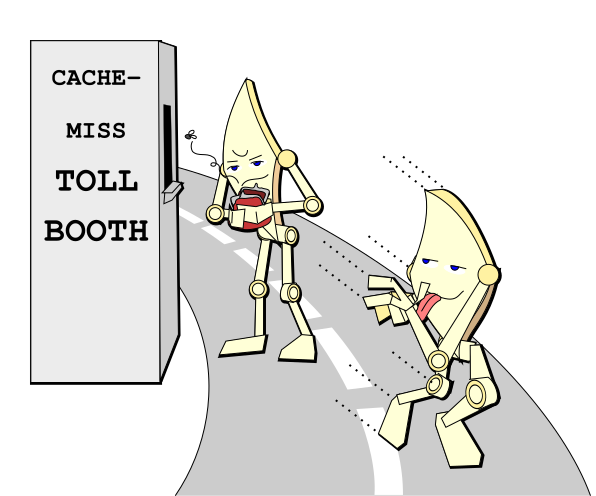
\includegraphics{cartoons/r-2014-CPU-track-meet-cache-miss-toll-booth}}
\caption{CPU遭遇Cache Miss}
\ContributedBy{fig:cpu:CPU Meets a Cache Miss}{Melissa Broussard}
\end{figure}

\subsection{I/O操作}
\label{sec:cpu:I/O Operations}

\begin{figure}
\centering
\resizebox{3in}{!}{\includegraphics{cartoons/r-2014-CPU-track-meet-phone-booth}}
\caption{CPU等待I/O完成}
\ContributedBy{fig:cpu:CPU Waits for I/O Completion}{Melissa Broussard}
\end{figure}

Cache miss可以视为CPU之间的I/O操作，
这应该是代价最低廉的I/O操作之一。
涉及网络、大容量存储器或（更糟的是）人类本身的I/O操作，
对性能的影响远远大于前几节提到的各种障碍，
如\cref{fig:cpu:CPU Waits for I/O Completion}所示。

这也是共享内存式的并行计算和分布式系统式的并行编程的一个不同点：
共享内存式并行编程的程序一般不会处理比cache miss更糟的情况，
而分布式并行编程的程序则很可能遭遇网络通信延迟。
这两种情况的延迟都可看作通信的开销——在顺序程序中所没有的开销。
因此，通信开销占实际执行工作量的比率是一项关键的设计参数。
并行硬件设计的一个主要目标是尽可能降低这个比率，
以达到性能和可扩展性上的目标。
反过来，正如将在\cref{chp:Partitioning and Synchronization Design}中看到的，
并行软件设计的一个主要目标是降低像cache miss这样的
昂贵操作的发生频率。

当然，说某个操作属于性能障碍是一方面，
说某个操作属于对性能影响非常\emph{显著}的障碍则是另一方面。
这一区别将在以下各节中讨论。

% cpu/overheads.tex
% mainfile: ../perfbook.tex
% SPDX-License-Identifier: CC-BY-SA-3.0

\section{开销}
\label{sec:cpu:Overheads}
%
\epigraph{不要在不了解材料的情况下设计桥梁，也不要在不了解底层硬件的情况下设计底层软件。}
	 {佚名}

本节将展示上一节列出的性能障碍的实际\IXpl{overhead}。
不过，首先需要对硬件系统架构有一个粗略的了解，这是下一节的主题。

\subsection{硬件系统架构}
\label{sec:cpu:Hardware System Architecture}

\begin{figure}
\centering
\resizebox{3in}{!}{\includegraphics{cpu/SystemArch}}
\caption{系统硬件架构}
\label{fig:cpu:System Hardware Architecture}
\end{figure}

\Cref{fig:cpu:System Hardware Architecture}
展示了一个八核计算机系统的概略示意图。
每个芯片包含一对CPU核心，每个核心都有自己的cache，
以及一个允许这对CPU相互通信的互连。
系统互连则允许四个芯片之间以及与主存之间进行通信。

数据以``\IXpl{cache line}''为单位在该系统中流动，
cache line是大小固定、地址对齐的2的幂次方内存块，
通常在32到256字节之间。
当CPU从内存加载一个变量到其寄存器时，
它必须首先将包含该变量的cache line加载到其cache中，
cache可以被视为一个硬件哈希表（hash table）。
类似地，当CPU将一个值从其寄存器存储到内存时，
它也必须将包含该变量的cache line加载到其cache中，
但还必须确保没有其他CPU拥有该cache line的副本。

\begin{figure}
\centering
\resizebox{3in}{!}{\includegraphics{cpu/SimpleWrite}}
\caption{一次``简单''存储的生命周期}
\label{fig:cpu:Lifetime of a Simple Store}
\end{figure}

例如，假设CPU~1向一个变量\co{x}写入，而该变量的cache line
在CPU~6的cache中。
结合\cref{fig:cpu:Lifetime of a Simple Store}，
以下过程的简化视图由这些步骤组成，
其中每一行都将\cref{fig:cpu:System Hardware Architecture}
简化为只显示CPU~1和~6、它们的store buffer和本地cache，
以及用灰色矩形表示的连接两个CPU的系统互连。

\begin{enumerate}
\item	CPU~1检查其本地cache，未找到该cache line。
	因此它将写操作记录在其store buffer中，
	如\cref{fig:cpu:Lifetime of a Simple Store}的A行所示。
\item	对该cache line的请求被转发到CPU~0和~1的互连，
	互连检查CPU~1的本地cache，未找到该cache line。
	由于没有任何变化，系统状态仍如
	\cref{fig:cpu:Lifetime of a Simple Store}的A行所示。
\item	该请求被转发到系统互连，
	如\cref{fig:cpu:Lifetime of a Simple Store}的B行所示，
	系统互连向其他三个芯片查询，
	得知该cache line由包含CPU~6和~7的芯片持有。
\item	该请求被转发到CPU~6和~7的互连，
	互连检查两个CPU的cache，在CPU~6的cache中找到了该值，
	如\cref{fig:cpu:Lifetime of a Simple Store}的C行所示。
\item	CPU~6将cache line转发给其互连，同时将该cache line
	从其cache中清除，然后CPU~6和~7的互连将cache line
	转发到系统互连，
	如\cref{fig:cpu:Lifetime of a Simple Store}的D行所示。
\item	系统互连将cache line转发到CPU~0和~1的互连，
	如\cref{fig:cpu:Lifetime of a Simple Store}的E行所示。
\item	CPU~0和~1的互连将cache line转发给CPU~1，
	如\cref{fig:cpu:Lifetime of a Simple Store}的F行所示。
\item	该cache line被存入CPU~1的cache中，
	如\cref{fig:cpu:Lifetime of a Simple Store}的G行所示。
\item	CPU~1现在可以完成写操作，用之前记录在store buffer中的值
	更新新到达的cache line的相关部分，
	如\cref{fig:cpu:Lifetime of a Simple Store}的H行所示。
\end{enumerate}

\QuickQuizSeries{%
\QuickQuizB{
	这是一个\emph{简化}的事件序列？
	它怎么\emph{可能}更复杂？
}\QuickQuizAnswerB{
	这个序列忽略了许多可能的复杂情况，包括：

	\begin{enumerate}
	\item	其他CPU可能正在并发地尝试对同一cache line执行
		内存引用操作。
	\item	该cache line可能已被只读复制到多个CPU的cache中，
		在这种情况下，需要从这些cache中清除。
	\item	当请求到达时，CPU~6可能正在操作该cache line，
		此时CPU~6可能需要暂缓请求，直到自己的操作完成。
	\item	CPU~6可能已经将该cache line从其cache中驱逐
		（例如，为了给其他数据腾出空间），
		因此当请求到达时，该cache line正在返回内存的途中。
	\item	cache line中可能发生了可纠正的错误，
		需要在数据被使用之前的某个时间点进行纠正。
	\end{enumerate}

	由于这些考虑因素，生产级的cache一致性机制极其
	复杂~\cite{Hennessy95a,DavidECuller1999,MiloMKMartin2012scale,DanielJSorin2011MemModel}。
%
}\QuickQuizEndB
%
\QuickQuizE{
	为什么必须从CPU~6的cache中清除该cache line？
}\QuickQuizAnswerE{
	如果不从CPU~6的cache中清除该cache line，
	那么CPU~1和~6可能对cache line中同一组变量持有不同的值。
	这种不一致性会极大地复杂化并行软件，
	因此明智的硬件架构师会避免这种情况。
}\QuickQuizEndE
}

这个简化的序列只是一门称为\emph{cache一致性协议}的
学科的开端~\cite{Hennessy95a,DavidECuller1999,MiloMKMartin2012scale,DanielJSorin2011MemModel}，
该协议在\cref{chp:app:whymb:Why Memory Barriers?}中有更详细的讨论\@。
从一个简单的内存写操作所触发的事件序列可以看出，
一条指令可能引发大量的协议流量，
这会显著降低你的并行程序的性能。

幸运的是，如果某个变量在一段时间内被频繁读取但从未被更新，
该变量可以被复制到所有CPU的cache中。
这种复制使所有CPU都能极快地访问这个\emph{读多写少}的变量。
\Cref{chp:Deferred Processing}介绍了充分利用这一重要的
硬件读多写少优化的同步机制。

\subsection{操作开销}
\label{sec:cpu:Costs of Operations}

\begin{table}
%\rowcolors{1}{}{lightgray}
\renewcommand*{\arraystretch}{1.1}
\centering\small
\tcresizewidth{
\begin{tabular}
  {
    ll
    S[table-format = 9.1]
    S[table-format = 9.1]
    r
  }
	\toprule
	\multicolumn{2}{l}{Operation}
			& \multicolumn{1}{r}{Cost (ns)}
				   & {\parbox[b]{.7in}{\raggedleft Ratio\\(cost/clock)}}
					    & CPUs \\
	\midrule
	\multicolumn{2}{l}{Clock period}
			   &   0.5 &    1.0 &		\\
	\midrule
	\multicolumn{2}{l}{Same-CPU}
			   &       &        & 0		\\
		& CAS      &   7.0 &   14.6 &		\\
		& lock     &  15.4 &   32.3 &		\\
	\midrule
	\multicolumn{2}{l}{On-Core}
			   &       &        & 224	\\
		& Blind CAS&   7.2 &   15.2 &		\\
		& CAS	   &  18.0 &   37.7 & 		\\
        \midrule
	\multicolumn{2}{l}{Off-Core}
			   &       &	    & 1--27	\\
		& Blind CAS&  47.5 &   99.8 & 225--251	\\
		& CAS	   & 101.9 &  214.0 &		\\
        \midrule
	\multicolumn{2}{l}{Off-Socket}
			   &       &        & 28--111	\\
		& Blind CAS& 148.8 &  312.5 & 252--335	\\
		& CAS	   & 442.9 &  930.1 &		\\
        \midrule
	\multicolumn{2}{l}{Cross-Interconnect}
			   &       &        & 112--223	\\
		& Blind CAS& 336.6 &  706.8 & 336--447	\\
		& CAS	   & 944.8 & 1984.2 &		\\
	\midrule
	\multicolumn{2}{l}{Off-System}
				&		&	      & \\
		& Comms Fabric  &         5 000 &      10 500 & \\
		& Global Comms  &   195 000 000 & 409 500 000 & \\
	\bottomrule
\end{tabular}
}
\caption{8 路 Intel Xeon Platinum 8176 @ 2.10\,GHz 系统中 CPU 0 视角的同步机制开销}
\label{tab:cpu:CPU 0 View of Synchronization Mechanisms on 8-Socket System With Intel Xeon Platinum 8176 CPUs at 2.10GHz}
\end{table}

对并行程序重要的一些常见操作的开销显示在
\cref{tab:cpu:CPU 0 View of Synchronization Mechanisms on 8-Socket System With Intel Xeon Platinum 8176 CPUs at 2.10GHz}中。
该系统的时钟周期约为0.5\,ns。
虽然现代微处理器在一个时钟周期内退役多条指令并不罕见，
但这些操作的开销仍然在第三列（标记为``Ratio''）中以时钟周期为单位进行了归一化。
关于这张表首先要注意的是，许多比率的值非常大。

同CPU的\acrmf{cas}操作消耗约7纳秒，
这个持续时间是时钟周期的十倍以上。
CAS是一种原子操作，硬件将指定内存位置的内容与指定的``旧''值进行比较，
如果相等，则存储指定的``新''值，此时CAS操作成功。
如果不相等，则内存位置保持其（意外的）值，CAS操作失败。
该操作是原子的，因为硬件保证在比较和存储之间
内存位置不会被更改。
在x86上，CAS功能由\co{lock;cmpxchg}指令提供。

``同CPU''前缀意味着当前对给定变量执行CAS操作的CPU也是最后一个访问
该变量的CPU，因此相应的cache line已经在该CPU的cache中。
类似地，同CPU的lock操作（由一次锁获取和一次锁释放组成的``往返''对）
消耗超过15纳秒，即超过30个时钟周期。
lock操作比CAS更昂贵，因为它需要对lock数据结构执行两次原子操作，
一次用于获取，另一次用于释放。

核内操作涉及共享同一核心的硬件线程之间的交互，
其开销与同CPU操作大致相同。
这并不令人惊讶，因为这两个硬件线程也共享完整的cache层次结构。

在blind CAS的情况下，软件在不查看内存位置的情况下指定旧值。
这种方法适用于尝试获取锁的场景。
如果未锁定状态用零表示，锁定状态用值一表示，
那么对lock执行CAS操作，指定零为旧值、一为新值，
如果锁尚未被持有，就会获取锁。
关键在于只有一次对内存位置的访问，即CAS操作本身。

相比之下，普通CAS操作的旧值来自于某个先前的load。
例如，要实现原子递增，先将共享变量的当前值加载到一个机器寄存器中，
然后递增以在另一个机器寄存器中产生新值。
然后在CAS操作中，第一个寄存器被指定为旧值，第二个寄存器被指定为新值。
如果共享变量的值在此期间没有变化，
CAS操作将存储新值，从而递增该共享变量。
然而，如果共享变量的值已经改变，旧值将不匹配，
导致比较失败，从而使CAS操作失败，不再对该共享变量做进一步更改。
关键在于现在有两次对内存位置的访问：load和CAS\@。

因此，核内blind CAS只消耗约7纳秒，
而核内CAS消耗约18纳秒，这并不令人意外。
非blind情况下额外的load并非免费的。
也就是说，这些操作的开销与同CPU的CAS和lock分别相似。

\QuickQuiz{
	\Cref{tab:cpu:CPU 0 View of Synchronization Mechanisms on 8-Socket System With Intel Xeon Platinum 8176 CPUs at 2.10GHz}
	显示CPU~0与CPU~224共享一个核心。
	然而，CPU 0与CPU 1共享一个核心不是更合理吗？
}\QuickQuizAnswer{
	对这种看法表示理解是很容易的，但文件
	\path{/sys/devices/system/cpu/cpu0/cache/index0/shared_cpu_list}
	中确实包含字符串\co{0,224}。
	因此，CPU~0的超线程伙伴确实是CPU~224。
	有人推测这种编号方式能让简单的应用程序和调度器表现更好，
	理由是在许多工作负载上第二个超线程并不能提供大量额外性能。
	这种推测假设简单的应用程序和调度器会按数字顺序使用CPU，
	将较弱的超线程伙伴CPU留到所有核心都在使用时才启用。
}\QuickQuizEnd

跨核（不同核心但在同一socket上）的blind CAS消耗近50纳秒，
即近100个时钟周期。
用于此cache miss测量的代码在一对CPU之间来回传递cache line，
因此此cache miss是从另一个CPU的cache中满足的，而不是从内存。
非blind CAS操作（如前所述，需要查看变量的旧值并存储新值）
消耗超过100纳秒，即超过200个时钟周期。
想一想这意味着什么。
在执行\emph{一次}CAS操作所需的时间里，CPU本可以执行
超过\emph{两百}条普通指令。
这应该能说明不仅是细粒度锁的局限性，
而且是任何依赖细粒度全局一致性的同步机制的局限性。

如果这对CPU分别在不同的socket上，操作就会昂贵得多。
一次blind CAS操作消耗近150纳秒，即超过300个时钟周期。
一次普通CAS操作消耗超过400纳秒，即近\emph{一千}个时钟周期。

更糟糕的是，并非所有socket对都是平等的。
这个特定系统似乎是由一对四socket组件构成的，
当CPU位于不同组件中时会有额外的延迟惩罚。
在这种情况下，一次blind CAS操作消耗超过300纳秒，
即超过700个时钟周期。
一次CAS操作消耗近一微秒，即近2000个时钟周期。

\QuickQuizLabelRel{\QspeedOfLightAtoms}{1} % cann't put label inside QQSeries

\QuickQuizSeries{%
\QuickQuizB{
	硬件设计师难道不能被说服改善这种状况吗？
	为什么他们对这些单指令操作如此低劣的性能感到满意？
}\QuickQuizAnswerB{
	硬件设计师\emph{一直}在致力于解决这个问题，
	并且咨询了不亚于已故物理学家Stephen Hawking这样的权威人物。
	Hawking的观察是，硬件设计师有两个基本
	问题~\cite{BryanGardiner2007}：

	\begin{enumerate}
	\item	有限的光速，以及
	\item	物质的原子性质。
	\end{enumerate}

\begin{table}
%\rowcolors{1}{}{lightgray}
\renewcommand*{\arraystretch}{1.1}
\centering\small
\begin{tabular}
  {
    ll
    S[table-format = 9.1]
    S[table-format = 9.1]
  }
	\toprule
	\multicolumn{2}{l}{Operation}
			& \multicolumn{1}{r}{Cost (ns)}
			& {\parbox[b]{.7in}{\raggedleft Ratio\\(cost/clock)}} \\
	\midrule
	\multicolumn{2}{l}{Clock period}
			&           0.4	&           1.0 \\
        \midrule
	\multicolumn{2}{l}{Same-CPU}
			&		&		\\
	& CAS		&          12.2	&          33.8 \\
	& lock		&          25.6	&          71.2 \\
        \midrule
        \multicolumn{2}{l}{On-Core}
			&		&		\\
	& Blind CAS	&          12.9	&          35.8 \\
	& CAS		&           7.0	&          19.4 \\
	\midrule
        \multicolumn{2}{l}{Off-Core}
			&		&		\\
	& Blind CAS	&          31.2	&          86.6 \\
	& CAS		&          31.2	&          86.5 \\
	\midrule
	\multicolumn{2}{l}{Off-Socket}
			&		&		\\
	& Blind CAS	&          92.4	&         256.7 \\
	& CAS		&          95.9	&         266.4 \\
	\midrule
	\multicolumn{2}{l}{Off-System}
			&		&		\\
	& Comms Fabric	&       2 600   &       7 220   \\
	& Global Comms	& 195 000 000	& 542 000 000   \\
	\bottomrule
\end{tabular}
\caption{16 核 2.8\,GHz Intel X5550 (Nehalem) 系统的同步机制性能}
\label{tab:cpu:Performance of Synchronization Mechanisms on 16-CPU 2.8GHz Intel X5550 (Nehalem) System}
\end{table}

	第一个问题限制了原始速度，第二个限制了小型化，
	而小型化反过来又限制了频率。
	而且这还没有考虑功耗问题，功耗目前将生产频率
	限制在远低于10\,GHz。

	此外，
	\cref{tab:cpu:CPU 0 View of Synchronization Mechanisms on 8-Socket System With Intel Xeon Platinum 8176 CPUs at 2.10GHz}
	（位于第~\cpageref{tab:cpu:CPU 0 View of Synchronization Mechanisms on 8-Socket System With Intel Xeon Platinum 8176 CPUs at 2.10GHz}页）
	代表的是一个相当大的系统，拥有不少于448个硬件线程。
	更小的系统通常能实现更低的延迟，如
	\cref{tab:cpu:Performance of Synchronization Mechanisms on 16-CPU 2.8GHz Intel X5550 (Nehalem) System}所示，
	该表代表一个只有16个硬件线程的小得多的系统。
	\cref{tab:cpu:CPU 0 View of Synchronization Mechanisms on 8-Socket System With Intel Xeon Platinum 8176 CPUs at 2.10GHz}
	中到``Off-Core''行（含该行）为止的各行也提供了类似的视角。

\begin{table}
%\rowcolors{1}{}{lightgray}
\renewcommand*{\arraystretch}{1.1}
\centering\small
\tcresizewidth{
\begin{tabular}
  {
    ll
    S[table-format = 9.1]
    S[table-format = 9.1]
    r
  }
	\toprule
	\multicolumn{2}{l}{Operation}
		& \multicolumn{1}{r}{Cost (ns)}
			& {\parbox[b]{.7in}{\raggedleft Ratio\\(cost/clock)}}
			& CPUs \\
	\midrule
	\multicolumn{2}{l}{Clock period}
				     &   0.5 &    1.0 &			  \\
        \midrule
	\multicolumn{2}{l}{Same-CPU} &       &        &	0		  \\
	& CAS			     &   6.2 &   13.6 &			  \\
	& lock			     &  13.5 &   29.6 &			  \\
        \midrule
	\multicolumn{2}{l}{On-Core}  &       &        &	6		  \\
	& Blind CAS		     &   6.5 &   14.3 &			  \\
	& CAS			     &  16.2 &   35.6 &			  \\
        \midrule
	\multicolumn{2}{l}{Off-Core} &       &        &	1--5		  \\
	& Blind CAS		     &  22.2 &   48.8 & 7--11		  \\
	& CAS			     &  53.6 &  117.9 &			  \\
	\midrule
	\multicolumn{2}{l}{Off-System}&       &        &		  \\
	& Comms Fabric		      & 5 000 & 11 000 &		  \\
	& Global Comms		      & 195 000 000 & 429 000 000 &	  \\
	\bottomrule
\end{tabular}
}
\caption{12 核 Intel Core i7-8750H @ 2.20\,GHz 系统中 CPU 0 视角的同步机制开销}
\label{tab:cpu:CPU 0 View of Synchronization Mechanisms on 12-CPU Intel Core i7-8750H CPU @ 2.20GHz}
\end{table}

	此外，较新的小规模单socket系统，
	如我正在键入本文的这台笔记本电脑，
	也具有更合理的延迟，如
	\cref{tab:cpu:CPU 0 View of Synchronization Mechanisms on 12-CPU Intel Core i7-8750H CPU @ 2.20GHz}所示。

	或者换个角度看，1990年代中期的一台64-CPU系统的跨互连延迟
	超过5微秒，因此即使是
	\cref{tab:cpu:CPU 0 View of Synchronization Mechanisms on 8-Socket System With Intel Xeon Platinum 8176 CPUs at 2.10GHz}
	中所示的那个八socket 448硬件线程的庞然大物，
	也比其25年前的同类产品改进了五倍以上。

	将硬件线程集成到单个核心中以及将多个核心集成到单个芯片上
	已经大大改善了延迟，至少在单个核心或单个芯片的范围内是如此。
	整个系统的延迟也有所改善，但仅约两倍。
	不幸的是，在过去几年里，光速和物质的原子性质
	并没有发生太大变化~\cite{NoBugsHare2016CPUoperations}。
	因此，空间和时间局部性是并发软件的首要关注点，
	即使在相对较小的系统上运行也是如此。

	\Cref{sec:cpu:Hardware Free Lunch?}
	将探讨硬件设计师还能做些什么来缓解并行程序员的困境。
}\QuickQuizEndB
%
\QuickQuizE{
	\Cref{tab:cpu:Performance of Synchronization Mechanisms on 16-CPU 2.8GHz Intel X5550 (Nehalem) System}
	（在第~\cpageref{tab:cpu:Performance of Synchronization Mechanisms on 16-CPU 2.8GHz Intel X5550 (Nehalem) System}页
	\QuickQuizARef{\QspeedOfLightAtoms}的答案中）
	显示核内CAS比同CPU的CAS和核内blind CAS都快。
	这是怎么回事？
}\QuickQuizAnswerE{
	我\emph{确实}对获得的数据感到惊讶，并对其有效性进行了严格验证。
	我持续得到了相同的结果。
	一个可能解释该观察结果的理论是：
	核心中的两个线程能够重叠其访问，
	而单个CPU必须顺序执行所有操作。
	遗憾的是，似乎没有公开文档解释Intel X5550 (Nehalem)系统
	为什么会表现出这种行为。
}\QuickQuizEndE
}                 % End of \QuickQuizSeries

\begin{table}
\rowcolors{1}{}{lightgray}
\renewcommand*{\arraystretch}{1.1}
\centering\small
\begin{tabular}{lrrrrr}
	\toprule
	Level &  Scope & Line Size &   Sets & Ways &    Size \\
	\midrule
	L0    &   Core &        64 &     64 &    8 &     32K \\
	L1    &   Core &        64 &     64 &    8 &     32K \\
	L2    &   Core &        64 &   1024 &   16 &   1024K \\
	L3    & Socket &        64 & 57,344 &   11 & 39,424K \\
	\bottomrule
\end{tabular}
\caption{8 路 Intel Xeon Platinum 8176 @ 2.10\,GHz 系统的缓存结构}
\label{tab:cpu:Cache Geometry for 8-Socket System With Intel Xeon Platinum 8176 CPUs @ 2.10GHz}
\end{table}

不幸的是，核内和socket内通信的高速度并非免费的。
首先，一个核心内只有两个CPU，一个socket内只有56个，
而整个系统有448个。
其次，如
\cref{tab:cpu:Cache Geometry for 8-Socket System With Intel Xeon Platinum 8176 CPUs @ 2.10GHz}所示，
核内cache与socket内cache相比非常小，
而socket内cache与该系统配置的1.4\,TB内存相比又非常小。
第三，再次参考该表，cache被组织为硬件哈希表，
每个桶只能容纳有限数量的条目。
例如，L3 cache的原始大小（``Size''）近40\,MB，
但每个桶（``Line''）只能容纳11个内存块（``Ways''），
每块最多64字节（``Line Size''）。
这意味着只需12字节的内存（当然是精心选择的地址）
就能使这个40\,MB的cache溢出。
另一方面，同样精心选择的地址可能会充分利用整个40\,MB。

空间局部性显然极其重要，数据在内存中的分散也同样重要。

I/O操作甚至更加昂贵。
如``Comms Fabric''行所示，
高性能（且昂贵！）的通信架构，如InfiniBand或众多专有互连，
端到端往返延迟约为5微秒，
在此期间可能已经执行了超过\emph{一万}条指令。
基于标准的通信网络通常需要某种协议处理，
这进一步增加了\IX{latency}。
当然，地理距离也会增加延迟，
光在光纤中绕地球一圈的光速延迟约为195\emph{毫秒}，
即超过4亿个时钟周期，
如\cref{tab:cpu:CPU 0 View of Synchronization Mechanisms on 12-CPU Intel Core i7-8750H CPU @ 2.20GHz}的``Global Comms''行所示。

% Reference for Infiniband latency:
% http://www.hpcadvisorycouncil.com/events/2014/swiss-workshop/presos/Day_1/1_Mellanox.pdf
%     page 6/76 'Leading Interconnect, Leading Performance'
% Needs updating...

\QuickQuiz{
	这些数字大得离谱！
	我怎么可能理解它们？
}\QuickQuizAnswer{
	拿一卷卫生纸。
	在美国，每卷通常有大约350--500张。
	撕下一张代表一个时钟周期，放到一边。
	现在展开剩下的纸卷。

	展开的那堆卫生纸大致代表一次\IXacr{cas} cache miss。

	对于更昂贵的系统间通信延迟，
	用几卷（或几箱）卫生纸来代表通信延迟。

	重要安全提示：
	在挪用卫生纸时，务必考虑到与你同住的人的需求，
	特别是在2020年或类似的时期，
	那时商店货架上的卫生纸和很多其他东西都被抢购一空。

	此外，对于从事内核代码工作的人来说，
	CPU在cache miss期间禁用中断，
	类似于你在展开一卷卫生纸时屏住呼吸。
	\emph{你}能在屏住呼吸的同时展开多少卷卫生纸？
	你可能需要避免在那么多次cache miss期间禁用中断。\footnote{
		感谢Matthew Wilcox提出这个屏住呼吸的类比。}
}\QuickQuizEnd

\subsection{硬件优化}
\label{sec:cpu:Hardware Optimizations}

自然会问硬件在这方面提供了什么帮助，答案是``相当多！''

一种硬件优化是大容量cache line。
这可以提供显著的性能提升，特别是当软件顺序访问内存时。
例如，给定64字节的cache line和软件访问64位变量，
第一次访问由于光速延迟（如果不是其他原因的话）仍然会很慢，
但剩余的七次可以非常快。
然而，这种优化有一个阴暗面，即\IX{false sharing}，
当同一cache line中的不同变量被不同的CPU更新时就会发生，
导致高cache miss率。\footnote{
	这种情况有时被称为``cache thrashing''
	或``cacheline bouncing''。}
软件可以使用许多编译器中提供的对齐指令来避免false sharing，
添加这样的指令是调优并行软件的常见步骤。

第二种相关的硬件优化是cache预取，
硬件对连续访问做出反应，预取后续的cache line，
从而避免这些后续cache line的光速延迟。
当然，硬件必须使用简单的启发式方法来确定何时预取，
而这些启发式方法可能被许多应用程序复杂的数据访问模式所欺骗。
幸运的是，一些CPU系列为此提供了特殊的预取指令。
不幸的是，这些指令在一般情况下的有效性仍然存在争议。

第三种硬件优化是store buffer，
它允许一串store指令快速执行，
即使这些store指向非连续地址且所需的cache line
都不在CPU的cache中。
这种优化的阴暗面是内存乱序，
详见\cref{chp:Advanced Synchronization: Memory Ordering}。

第四种硬件优化是推测执行，
它可以让硬件充分利用store buffer而不导致内存乱序。
这种优化的阴暗面可能是能源效率低下和
当推测执行出错需要回滚重试时性能降低。
更糟糕的是，Spectre和Meltdown~\cite{JannHorn2018MeltdownSpectre}
的出现表明，硬件推测还可能使侧信道攻击成为可能，
这些攻击能击败内存保护硬件，
使无特权进程读取它们不应访问的内存。
显然，推测执行与云计算的结合需要相当多的改进！

有人可能会争辩说，如果人们能合理行事，
侧信道攻击的缓解措施就不是必需的。
然而，远程可访问的计算机系统确实经常受到
有组织犯罪和国家行为体的攻击，
更不用说无聊的青少年了。
有句老话说``少数人就能搞砸所有人的事''，
但现实是远程可访问的计算机系统必须被积极地防御攻击。

第五种硬件优化是大容量cache，
允许单个CPU在更大的数据集上操作而不产生昂贵的cache miss。
虽然大容量cache可能会降低\IXh{energy}{efficiency}和
\IXh{cache-miss}{latency}，
但生产微处理器上不断增长的cache大小证明了这种优化的强大。

最后一种硬件优化是读多写少的复制，
其中被频繁读取但很少更新的数据存在于所有CPU的cache中。
这种优化允许极其高效地访问读多写少的数据，
是\cref{chp:Deferred Processing}的主题。

\begin{figure}
\centering
\resizebox{3in}{!}{\includegraphics{cartoons/Data-chasing-light-wave}}
\caption{硬件与软件：并肩作战}
\ContributedBy{fig:cpu:Hardware and Software: On Same Side}{Melissa Broussard}
\end{figure}

简而言之，硬件工程师和软件工程师实际上是站在同一边的，
都在努力让计算机跑得更快，尽管物理定律竭尽全力加以阻挠，
如\cref{fig:cpu:Hardware and Software: On Same Side}
中所夸张描绘的那样，其中我们的数据流正竭尽全力超越光速，
还受到非零原子大小的进一步阻碍。
下一节将讨论硬件工程师可能（也可能无法）做的一些额外事项，
这取决于近期研究转化为实践的程度。
软件对这一崇高目标的贡献将在本书其余章节中概述。

% cpu/hwfreelunch.tex
% mainfile: ../perfbook.tex
% SPDX-License-Identifier: CC-BY-SA-3.0

\section{硬件的免费午餐？}
\label{sec:cpu:Hardware Free Lunch?}
%
\epigraph{当今最大的问题是有太多人在寻找别人来为自己做些什么。
	  大多数问题的解决之道在于每个人为自己做些什么。}
	 {Henry Ford，改编}

近年来并发性受到如此多关注的主要原因是
\IXaltr{Moore's-Law}{Moore's Law}驱动的单线程性能提升
（或曰``免费午餐''~\cite{HerbSutter2008EffectiveConcurrency}）的终结，
如\cref{fig:intro:Clock-Frequency Trend for Intel CPUs}
（第~\cpageref{fig:intro:Clock-Frequency Trend for Intel CPUs}页）所示。
本节简要介绍硬件设计师可能采用的一些办法，
这些办法可以带来某种形式上的``免费午餐''。

然而，前一节展示了利用并发性所面临的一些重大硬件障碍。
其中对硬件设计师来说最严重的一个限制莫过于有限的光速。
如\cref{fig:cpu:System Hardware Architecture}
（第~\cpageref{fig:cpu:System Hardware Architecture}页）所述，
在1.8\,GHz的时钟周期内，光在真空中只能传播约8厘米远。
对于5\,GHz时钟，这个距离更是降到约3厘米。
这两个距离对于一个现代计算机系统的尺寸来说，还是太小了点。

更糟糕的是，电子在硅中的移动速度是真空中光速的1/30到1/3，
而常见的时钟逻辑结构运行得更慢。例如，
一次内存引用可能需要等待本地cache查找完成后才能将请求传递给系统的其余部分。
此外，将电信号从一个硅芯片传输到另一个（例如CPU与主存之间的通信）
需要相对低速且高功耗的驱动器。

\QuickQuiz{
	但单个电子的移动速度远没有那么快，即使在导体中也是如此！
	在半导体电压水平下，导体中电子的漂移速度仅为每秒
	约一\emph{毫米}。
	这是怎么回事？
}\QuickQuizAnswer{
	电子漂移速度追踪的是单个电子的长期运动。
	事实上，单个电子的运动相当随机，
	因此它们的瞬时速度很高，
	但从长期来看，它们并没有移动多远。
	在这一点上，电子类似于长途通勤者，
	他们可能大部分时间以全高速公路速度行驶，
	但从长期来看却哪里也没去。
	这些通勤者的速度可能是每小时70英里（每小时113公里），
	但他们相对于地球表面的长期漂移速度是零。

	因此，我们应该关注的不是电子的漂移速度，
	而是它们的瞬时速度。
	然而，即使是它们的瞬时速度也远不及光速的很大一部分。
	尽管如此，导体中电波的实测速度\emph{确实}是光速的相当大一部分，
	所以我们手头仍有一个谜。

	另一个诀窍是，电子之间在相当大的距离上
	（至少从原子的角度来看）相互作用，
	这要归功于它们的负电荷。
	这种相互作用由光子承载，而光子\emph{确实}以光速运动。
	所以即使在电学中的电子那里，
	大部分高速工作也是由光子完成的。

	推广通勤者的类比，一个司机可能使用智能手机
	通知其他司机有关事故或拥堵的情况，
	从而使交通流量的变化传播速度远快于
	单个汽车的瞬时速度。
	总结电学与交通流的类比：

	\begin{enumerate}
	\item	电子的（非常低的）漂移速度类似于通勤者的长期速度，
		两者都非常接近于零。
	\item	电子的（仍然相当低的）瞬时速度类似于
		交通中汽车的瞬时速度。
		两者都远高于漂移速度，
		但与变化传播速度相比仍然很小。
	\item	电波的（高得多的）传播速度主要是由于光子
		在电子之间传递电磁力。
		同样，由于司机之间的通信，
		交通模式可以相当快地改变。
		当然，这对已经堵在路上的司机不一定有多大帮助，
		就像对已经聚集在某个电容器中的电子一样。
	\end{enumerate}

	要完全理解这个主题，请学习电动力学。
}\QuickQuizEnd

事实上，据说Stephen Hawking曾声称半导体制造商面临两个基本问题：
\begin{enumerate*}[(1)]
\item 有限的光速，以及
\item 物质的原子性质~\cite{BryanGardiner2007}。
\end{enumerate*}
没错，光太慢而原子太大！

尽管如此，仍有一些技术（包括硬件和软件）可能有助于改善现状：

\begin{enumerate}
\item	新型材料和工艺，
\item	用光代替电，
\item	3D集成，
\item	专用加速器，以及
\item	现有的并行软件。
\end{enumerate}

以下各节分别介绍上述每一项。

\subsection{新型材料和工艺}
\label{sec:cpu:Novel Materials and Processes}

半导体制造商很有可能已经逼近了有限光速和
非零原子尺寸所隐含的极限。
然而，仍有一些研究和开发方向致力于绕过这些基本物理定律。

其中一个规避物质原子性质的办法是一种称为``高K介电''的材料，
这种材料允许较大的器件模拟不可行的微小器件的电学特性。
这些材料存在一些严峻的制造困难，
但仍然可能有助于将前沿推得更远一些。
另一种比较奇特的变通方法是在单个电子中存储多个比特，
利用给定电子可以存在于多个能量级别的事实。
这种特定方法能否在量产半导体器件中稳定工作还有待观察。

另一种提出的变通方法是``量子点''方法，
它允许更小的器件尺寸，但仍处于研究阶段。
还有一种提出的变通方法是用真空代替传统晶体管底部的原子，
从而得到真空间隙晶体管。

一个挑战是，许多最近的硬件器件级突破
需要非常精确地控制哪个原子放在
哪里~\cite{MichaelJKelly2017DeviceLevel}。
因此，找到在芯片上数十亿个器件中逐个放置原子的好方法的人，
即使别无所获，至少也能获得最出色的吹牛资本！

\subsection{光，而非电子}
\label{sec:cpu:Light; Not Electrons}

虽然光速是一个很难逾越的限制，但半导体设备更多是受限于电子移动的速度，
而非光速本身。半导体材料中电波的传播速度仅为
真空光速的3\pct 到30\pct。
在硅质器件上使用铜导线是一种提升电传播速度的方法，
而且很有可能进一步的进展将让电传播速度更加接近实际光速。
此外，已经有一些实验使用微型光纤作为芯片内部和芯片之间的传输通道，
因为在玻璃中光速能达到真空光速的60\pct 甚至更多。
这种方法存在的一个问题是光电/电光转换的效率，
会产生功耗和散热问题。

不仅如此，在物理学领域没有突破性进展的情况下，
数据流传输速度的任何指数增长都将受到真空光速的严格限制。

\subsection{3D集成}
\label{sec:cpu:3D Integration}

三维集成（3DI）是将非常薄的硅芯片垂直堆叠粘合在一起的工艺。
这项工艺带来了一些潜在的好处，但也带来了
重大的制造挑战~\cite{JohnKnickerbocker2008:3DI}。

\begin{figure}
\centering
\resizebox{3in}{!}{\includegraphics{cpu/3DI}}
\caption{3D集成的延迟优势}
\label{fig:cpu:Latency Benefit of 3D Integration}
\end{figure}

也许3DI所带来的最大好处是降低了系统的路径长度，
如\cref{fig:cpu:Latency Benefit of 3D Integration}所示。
一个3厘米的硅芯片可以被四块重叠的1.5厘米芯片替代，
要知道每一层都非常薄。
不仅如此，如果能小心地设计和加工，
长的水平方向电连接（既慢又耗电）可以被短的垂直方向电连接所取代，
后者既更快又更节能。

如果你不能让光跑得更快，就把你的器件做得更小！

不过，时钟逻辑结构级别造成的延迟是无法通过3D集成来降低的，
并且诸如生产、测试、供电和散热等3D集成中的重大问题
必须得到解决才有望产品化。
散热问题可能需要用基于金刚石的半导体来解决，
金刚石是热的良好导体，但却是电的绝缘体。
据说生长大尺寸的单晶金刚石仍然很困难，
更别说将金刚石切割成晶圆了。
不仅如此，上述这些技术看起来不大可能像某些人习惯的那样让性能出现指数级增长。
不过，它们可能是通往已故Jim Gray所说的
``冒烟的毛茸茸的高尔夫球''~\cite{JimGray2002SmokingHairyGolfBalls}道路上的必要步骤。

\begin{figure}
\centering
\resizebox{3in}{!}{\includegraphics{cpu/High_Bandwidth_Memory_schematic}}
\caption{3D集成示例}
\ContributedBy{fig:cpu:Example 3D Integration}{Shmuel Csaba Otto Traian, CCSA4.0}
\end{figure}

与此同时，大约2020年，chiplet\footnote{
	\url{https://en.wikipedia.org/wiki/Chiplet}}
技术的进步在这个方向上取得了重大进展，
如\cref{fig:cpu:Example 3D Integration}所示。
一些研究人员正在更进一步，在单个芯片内堆叠
晶体管~\cite{SamuelKMoore2020StackedCMOS,MarkoRadosavljevic2022StackedCMOS}。

\subsection{专用加速器}
\label{sec:cpu:Special-Purpose Accelerators}

用通用CPU来处理某个专门问题，通常会将大量的时间和能源消耗
在和问题无关的地方。
例如，当对一对向量进行点积操作时，通用CPU一般会使用一个循环
（通常已展开）和一个循环计数器。
对指令解码、递增循环计数器、测试计数器以及跳转回循环顶部，
从某种意义上来说都是无用功：
真正的目标是计算两个向量对应元素的乘积。
因此，在硬件上设计一个专用于向量乘法的部件
可以让这项工作完成得既快速又节能。

这就是在许多商用微处理器上出现向量指令的原因。
这些指令可以同时操作多个数据，
能让点积计算减少指令解码和循环开销的消耗。

类似地，专用硬件可以更有效地进行加密/解密、
压缩/解压缩、编码/解码等许多任务。
不过不幸的是，这种效率提升并非免费的。
包含专用硬件的计算机系统将需要更多的晶体管，
即使在不用时也会带来能源消耗。
软件也必须进行修改以利用专用硬件的长处，
同时这种专用硬件又必须有足够广泛的通用性，
这样高昂的前期设计费用才能摊到足够多的用户身上，
让专用硬件的价格变得可以承受。
部分由于以上经济考虑因素，专用硬件迄今只出现在少数
应用领域，包括图形处理（GPU）、向量处理器（MMX、SSE
和VMX指令），以及在较小程度上的加密和压缩。
即使在这些领域，实现预期的性能提升也并非总是容易的，
例如，由于热节流~\cite{VladKrasnov2017SIMDfreqscale,DanielLemire2018SIMDfreqscale,TravisDowns2020SIMDfreqscale}。

与服务器和PC领域不同，智能手机长期以来使用了
各种各样的硬件加速器。
这些硬件加速器通常用于媒体解码，
以至于一个高端MP3播放器可能能够播放数分钟的音频——
其CPU在整个过程中完全断电。
这些加速器的目的是提高能源效率从而延长电池寿命：
专用硬件通常可以比通用CPU更高效地进行计算。
这是\cref{sec:intro:Generality}中指出的原则的又一个例子：
\IX{Generality}几乎从来都不是免费的。

尽管如此，鉴于\IXaltr{Moore's-Law}{Moore's Law}驱动的
单线程性能提升的终结，可以安全地假设将会出现越来越多种类的专用硬件。
例如，在2020年代中期，许多人押注于专用于人工智能和
机器学习工作负载的加速器。

\subsection{现有的并行软件}
\label{sec:cpu:Existing Parallel Software}

虽然多核CPU曾经让计算行业惊讶了一把，
但事实上基于共享内存的并行计算机至少从1980年代起
就已经随时可用（尽管价格不菲）。
这段时间足以让一些重要的并行软件登上舞台，
事实也确实如此。
并行操作系统已经非常常见，并行线程库、
并行关系数据库管理系统和并行数值软件也是如此。
这些现有的并行软件在解决我们可能遇到的并行难题上已经走了很长一段路。

也许最常见的例子是并行关系数据库管理系统。
与单线程程序不同，并行关系数据库管理系统一般用高级脚本语言书写，
并发地访问位于中心的关系数据库。
在这种高度并行化的系统中，只有数据库本身需要直接处理并行性。
当这种方式奏效时，真是一个非常好的技巧！

% cpu/swdesign.tex
% mainfile: ../perfbook.tex
% SPDX-License-Identifier: CC-BY-SA-3.0

\section{软件设计启示}
\label{sec:cpu:Software Design Implications}
%
\epigraph{一船向东行，一船向西驶，\\
	  吹的却是同样的风；\\
	  决定航向的不是风的力量，\\
	  而是帆的方向。}
	 {Ella Wheeler Wilcox}

\cref{tab:cpu:CPU 0 View of Synchronization Mechanisms on 8-Socket System With Intel Xeon Platinum 8176 CPUs at 2.10GHz}
中比率的数值至关重要，因为它们限制了并行应用程序的效率。
为了弄清这一点，我们假设一款并行程序使用\IXacr{cas}操作来进行线程间通信。
假设进行通信的线程不是与自身而是主要与其他线程通信，
那么CAS操作通常会涉及cache miss。
进一步假设对应每次CAS通信操作的工作需要消耗300\,ns，
这足以计算几个浮点超越函数。
其中一半的执行时间将消耗在CAS通信操作上，
这也意味着两个CPU的系统运行这样一个并行程序的速度，
并不比单CPU系统运行一个串行程序的速度快。

在分布式系统的情况下结果还会更糟，
因为单次通信操作的延迟可能和数千甚至数百万次
浮点运算所需的时间一样长。
这也说明了通信操作应该尽力避免，每次通信应该能够处理大量数据。

\QuickQuiz{
	既然分布式系统的通信如此昂贵，
	为什么还有人费心使用这样的系统？
}\QuickQuizAnswer{
	原因有很多：

	\begin{enumerate}
	\item	共享内存多处理器系统有严格的规模限制。
		如果你需要超过几千个CPU，就别无选择，
		只能使用分布式系统。
	\item	大型共享内存系统的每单位计算成本
		往往高于小型系统。
	\item	大型共享内存系统的cache miss延迟
		往往比小型系统大得多。
		要看到这一点，请比较
		\cref{tab:cpu:CPU 0 View of Synchronization Mechanisms on 8-Socket System With Intel Xeon Platinum 8176 CPUs at 2.10GHz}
		（第~\cpageref{tab:cpu:CPU 0 View of Synchronization Mechanisms on 8-Socket System With Intel Xeon Platinum 8176 CPUs at 2.10GHz}页）
		和\cref{tab:cpu:CPU 0 View of Synchronization Mechanisms on 12-CPU Intel Core i7-8750H CPU @ 2.20GHz}。
	\item	分布式系统的通信操作不一定消耗太多CPU，
		因此计算可以与消息传输并行进行。
	\item	许多重要问题是``令人尴尬的并行''，
		因此极少量的消息就能启用极大量的处理。
		SETI@HOME~\cite{SETIatHOME2008}
		就是此类应用的一个例子。
		这类应用即使在通信延迟极长的情况下，
		也能很好地利用计算机网络。
	\end{enumerate}

	因此，大型共享内存系统往往用于那些受益于比分布式计算
	所能提供的更快延迟的应用，
	特别是那些受益于大共享内存的应用。

	继续进行的并行应用研究工作很可能会增加能够在
	通信延迟较长的机器和/或集群上良好运行的令人尴尬的并行
	应用的数量，降低成本是推动这一趋势的驱动力。
	话虽如此，大幅降低硬件延迟将是一个极受欢迎的发展，
	无论是对于单系统还是分布式计算。
	事实上，这样的降低正在发生，
	尽管从我们这些经历过2000年代初期之前
	CPU时钟频率指数增长的人的角度来看，速度相当缓慢。
}\QuickQuizEnd

这一课应该非常明了：
并行算法必须将每个线程设计成尽可能独立运行的线程。
越少使用线程间通信手段——比如\IX{atomic}操作、lock或者其他消息传递方法——
应用程序的性能和可扩展性就越好。
这种方法将在\cref{chp:Counting}中初步涉及，
在\cref{chp:Partitioning and Synchronization Design}中深入探讨，
并在\cref{chp:Data Ownership}中推向其逻辑极致。

另一种方法是确保任何共享都是读多写少的，
这允许CPU的cache复制读多写少的数据，
从而使所有CPU都能快速访问。
这种方法在\cref{sec:count:Eventually Consistent Implementation}中初步涉及，
并在\cref{chp:Deferred Processing}中更深入地探讨。

简而言之，想要达到优秀的并行性能和可扩展性，
就意味着在并行算法和实现中努力追求，
无论是通过精心选择数据结构和算法、利用现有的并行软件和环境，
还是将并行问题转化为已经有并行解决方案存在的问题。

\QuickQuiz{
	好吧，如果我们不得不将分布式编程技术
	应用于共享内存并行程序，
	那为什么不总是使用这些分布式技术而抛弃共享内存呢？
}\QuickQuizAnswer{
	因为通常情况下，只有一小部分程序是性能关键的。
	共享内存并行性允许我们将分布式编程技术
	集中在那一小部分上，
	而在非性能关键的大部分程序上使用更简单的共享内存技术。
}\QuickQuizEnd


总结一下：

\begin{enumerate}
\item	好消息是，多核系统价格低廉且随处可得。
\item	更多好消息：
	许多同步操作的开销比2000年代初期的并行系统要低得多。
\item	坏消息是，cache miss的开销仍然很高，尤其是在大型系统上。
\end{enumerate}

本书的其余部分将介绍应对这一坏消息的方法。

具体而言，
\cref{chp:Tools of the Trade}将介绍一些用于并行编程的底层工具，
\cref{chp:Counting}将探讨并行计数的问题和解决方案，
\cref{chp:Partitioning and Synchronization Design}将讨论促进性能和可扩展性的设计原则。

\QuickQuizAnswersChp{qqzcpu}
